\section{Gradient-based opacity weighting}\label{Sec:Gow}
Another task was to implement gradient-based opacity weighting in our raycaster.
We used the gradient-based opacity as described in Levoy’s paper.
Gradient-based opacity is useful when there is more than one type of  material in the scene. 
Gradient-based opacity can then be used to display or hide certain materials.
With this function we can compute the new opacity value for each pixel:
\[ \tau(i) = |\bigtriangledown f_{i}| \left\{
  \begin{array}{lr}
   \tau_{min} (\frac{ f_{max}- f_{i}}{ f_{max}- f_{min}}) +\tau_{max}( \frac{ f_{i}- f_{min}}{ f_{max}- f_{min}})  & : f_{min} \leq f_{i}  \leq f_{max} \\
    0 & : otherwise 
  \end{array}
\right.
\] 
We can approximate the gradient in the same way we would do this in one dimension. 
In one dimension we would look at i+1 and i-1 and compute a gradient with those two values.
When we do this in three dimensions, we have to look at all points +1 and -1 in that dimension.
So we can estimate the gradient with these function:
$$\bigtriangledown f_{i} = ( 
\frac{ 1}{2}( f_{x_{i+1},y_{j},z_{k}},f_{x_{i-1},y_{j},z_{k}} ),
\frac{ 1}{2}( f_{x_{i},y_{j+1},z_{k}},f_{x_{i},y_{j-1},z_{k}} ),
\frac{ 1}{2}( f_{x_{i},y_{j},z_{k+1}},f_{x_{i},y_{j},z_{k-1}} )) $$
Because we do not know these values, we have made a settings box that enables users to easily play with those values.
In figure~\ref{fig:gradient_settings} you can see those settings. 
As you can see we added another option: Factor. 
By changing the factor, the user can increase or decrease the effect of the gradient-based opacity weighting function.
\begin{figure}[H]
	\centering
		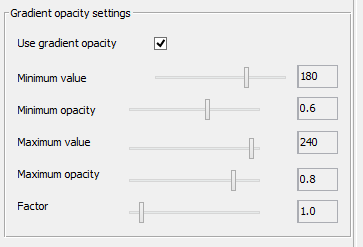
\includegraphics[width=0.4\textwidth]{gradient_settings}
		\caption{Settings for the gradient-based opacity weighting}
	\label{fig:gradient_settings}
\end{figure}
As you can see in figure~\ref{fig:gradient} we can eliminate all other materials and just show the bones.
We made the bones blue, so they are better visible on a white background. 
\begin{figure}[H]
	\centering
		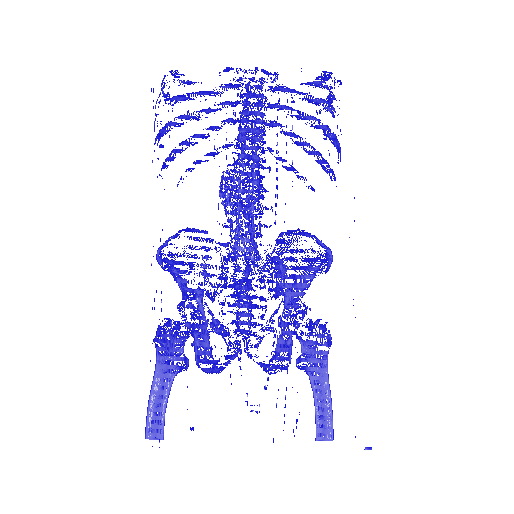
\includegraphics[width=0.6\textwidth]{stent_with_gradient}
		\caption{Only the bones of \texttt{stent8.fld}}
	\label{fig:gradient}
\end{figure}